\section{G-mašine}
\label{sec:Gmasine}

U ovom delu predstavićemo {\em G mašinu} (eng. G-machine), koju su Avgustson i Džonson (eng. Augustsson and Johnsson) predstavili u svojim naučnim radovima, na Tehnološkom institutu Čalmers (eng. Chalmers Institute of Technology) u Geteburgu, između 1984. i 1987. godine. 

\subsection{Motivacija}
Kod {\em lenjih funkcionalnih jezika} funkcije i argumenti konstruktora se evaluiraju samo po potrebi, pa čak i onda najviše samo jednom. \\
\\Bez obzira na to što se ovako nešto može implementirati predstavljanjem neevaluiranih argumenata "tankovima" (eng. thunk) - funkcijom koja evaluira argument i zamenjuje ga rezultatom, zbog efikasnosti biramo drugačije pristupe. \\Osnovna ideja je da predstavimo program {\em grafom} koji bismo kasnije "prepisali"  evaluacijom. Velika prednost je i u tome što evaluacija deljenog podgrafa automatski razrešava sve izraze koji pokazuju na njega. Međutim, treba biti pažljiv, kontinuirana pretraga grafa za podizrazima je {\em spora}. \\\\
Rane implementacije su prevodile program u fiksirani skup kombinatora (zatvorene lambda izraze čije su apstrakcije na početku), koje možemo posmatrati kao pravila za "prepisivanje grafa". Kasnije se pokazalo da je korisno prepustiti programu da razmatra izbor kombinatora - tzv. {\em superkombinatora}. \\ %ovde ide ova ref ] R.J.M. Hughes, Super-combinators: A new implementation method for applicative languages, ACM Symposium on Lisp and Functional Programming, Pittsburgh, Pennsylvania,ACM, August 1982, pp. 1–10.1


\subsection{Osnovna ideja} 
Umesto da interpretiraju superkombinatore kao pravila za prepisivanje grafa, oni se kompajliraju u kod sa specijalnim instrukcijama za manipulaciju grafom. G-mašine su osnova implementacije lenjog ML (eng. lazy ML) i Haskela. 
%uz Lazy ML ide L. Augustsson, The interactive lazy ML system, J. Funct.Programming 3 (1) (1993) 77–92, A UZ HASKEL ] L. Augustsson, HBC – The Chalmers Haskell compiler,Web Page, 1999, URL: http://www.cs.chalmers.se/augustss/hbc.html.

Sada ćemo navesti osnovnu ideju koja stoji iza G-mašina: \\
\textbf{{\em Pre pokretanja programa, svako telo superkombinatora treba da se prevede u niz instrukcija koje, nakon što se izvrše, kreiraju instancu tela superkombinatora.}}\\

Uvek želimo samo da instanciramo superkombinator, tako da možemo da obacimo originalne superkombinatore nakon što je prevođenje završeno, i sačuvamo samo preveden kod. Dakle, koristimo kompajler G-mašine da izvorni kod prevedemo u niz instrukcija na mašinskom jeziku. \\

Nakon što smo odlučili da prevedemo telo superkombinatora u niz instrukcija moramo da odlučimo u koji jezik ćemo da ga prevedemo. Iako bismo mogli da ga odmah prevedemo u, na primer, {\em VAX mašinski kod}, kasnije bi nam se javili mnogi problemi.\\
Najbolje rešenje, ujedno i ono koje se najčešće koristi, je da prevođenje izvršimo u središnji kod (eng. intermediate code) za G-mašinu, takozvani G-kod (eng. G-code). \\

\subsection{G-kod}

{\em G-kod} je kod u koji kompajliramo tela superkombinatora, kompilator za G-mašinu prati sledeći niz postupaka:
\begin{enumerate}
\item Izvorni jezik je varijanta ML-a, sa semantikom lenje evaluacije, tzv. {\em lenji ML}.
\item Rane faze kompilacije vrše proveru tipova, nalaženje uzoraka i analizu zavisnosti. U ovoj fazi program je preveden na $\lambda$-račun.
\item $\lambda$-lifter (eng. $\lambda$-lifter) transformiše program u oblik superkombinatora.   
\item Superkombinatori se prevode u G-kod.
\item Konačno, generiše se mašinski kod iz G-koda za ciljnu mašinu.
\end{enumerate}
%referenca za G kompajler Peyton Jones, Simon L., 1958-The implementation of functional programming languages.'7th May 1986.'Bibliography: p.Includes index.I. Functional programming languages. I. Title.QA76.7.P495 1987 005.13'3 86-20535 ISBN 0-13-453333-X
\begin{figure}[h!]
\begin{center}
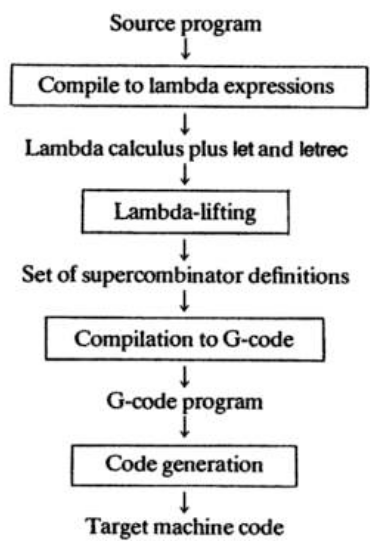
\includegraphics[scale=0.4]{gkomp.png}
\end{center}
\caption{Struktura G-kompajlera}
\label{fig:gcompiler}
\end{figure}
%referenca za primer i vise info o G masinama Implementing Functional Languages:a tutorial Simon L Peyton Jones Department of Computing Science, University of Glasgow and David R LesterDepartment of Computer Science, University of Manchesterc 1991
\begin{primer}
Predstavimo sad način na koji funkcioniše kompajler za G mašinu razmatrajući sledeću funkciju:\\
f g x = K (g x)\\
Ova funkcija bi se prevela u sledeći niz instrukcija G-koda:
\begin{itemize}
\item Push 1
\item Push 1
\item Mkap
\item Pushglobal K
\item Mkap
\item Slide 3
\item Unwind
\end{itemize}
\end{primer}

Na slici \ref{fig:primerGmasine} prikazujemo kako se kod izvršava.\\
Sa leve strane svakog dijagrama prikazan je stek, koji raste na dole. Ostatak svakog dijagrama je hip. Aplikativni čvorovi predstavljeni sa karakterom @, izrazi sa malim slovima, a superkombinatori sa velikim slovima latinice.\\ 
Na slici \ref{fig:primerGmasine} prikazano je stanje mašine pre izvođenja instrukcija za f. Dva elementa na vrhu steka su pokazivači na aplikativne čvorove, čije su desne strane izrazi koji će biti vezani za g i x.\\ 
Instrukcija Push koristi relativno adresiranje u odnosu na vrh steka. Ignorišući pokazivač na supekombinatorski čvor f, prvi element na steku dobija broj 0, naredni 1, itd..\\ 
Naredni dijagram (b) pokazuje kako se stek izmenio nakon primene Push1 instrukcije. Ona stavlja pokazivač na izraz x na stek. \\ Nakon jos jednog izvršavanja Push1 instrukcije, imamo pokazivač na g na vrhu steka i onda imamo ono što je prikazano na dijagramu (c). \\ Dijagram (d) pokazuje šta se dešava kada se izvrši Mkap instrukcija. Ona uzima dva pokazivača sa steka i pravi aplikativni čvor, ostavljajući pokazivač na rezultat na steku. \\ Na dijagramu (e) izvršavamo Pushglobal K instukciju koja stavlja pokazivač na K superkombinator. \\ Na dijagramu (f) vidimo da još jedna Mkap instrukcija završava instanciranje tela f.\\ 
Sada možemo zameniti originalni izraz f g x  sa novoinstanciranim telom: K(g x). U prvoj (ne lenjoj) verziji G-mašine, jednostavno pomerimo telo na dole za 3 mesta na steku pomoću instrukcije Slide 3 (dijagram (g)).\\ Konačno, Unwind instrukcija uzrokuje dalju evaluaciju.\\
\begin{figure}[h!]
\begin{center}
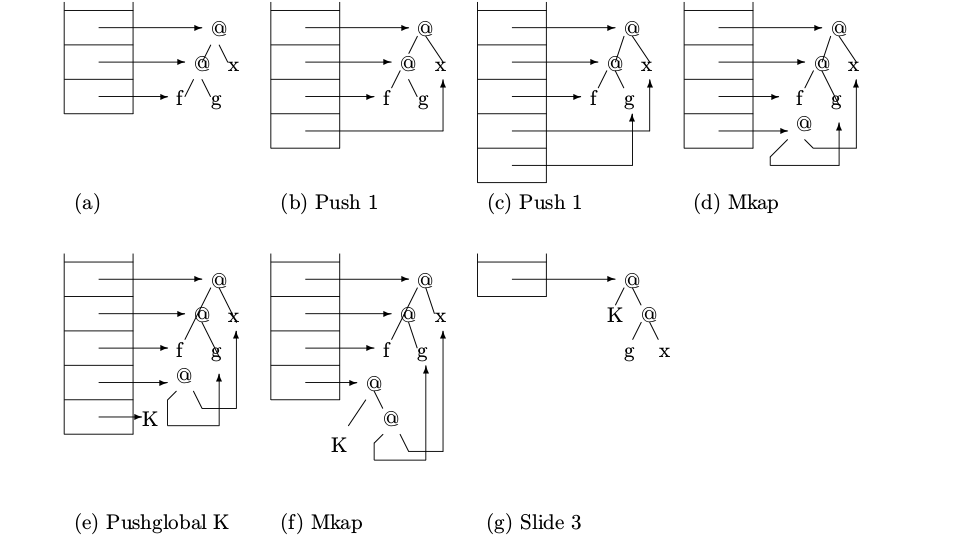
\includegraphics[scale=0.35]{primerGmasine.png}
\end{center}
\caption{Vizuelni prikaz}
\label{fig:gcompiler}
\end{figure}
%za sve ref dodati Abstract machines for programming language implementation Stephan Diehl a,∗, Pieter Hartel b, Peter Sestoft c a FB-14 Informatik, Universität des Saarlandes, Postfach 15 11 50, 66041 Saarbrücken, Germany b Department of Electronics and Computer Science, University of Southampton, Highfield, Southampton SO17 1BJ, UK c Department of Mathematics and Physics, Royal Veterinary and Agricultural University, Thorvaldsensvej 40,DK-1871 Frederiksberg C, Denmark Accepted 24 June 1999

\addcontentsline{toc}{section}{Literatura}
\appendix
\bibliography{seminarski} 
\bibliographystyle{plain}

\appendix

\end{document}
